\documentclass{article}
\usepackage[utf8]{inputenc}
\usepackage[T1]{fontenc}
%\usepackage[euler-digits,euler-hat-accent]{eulervm}
%\usepackage{concrete}
\usepackage{amsmath}
\usepackage{graphicx}
\usepackage{amssymb}
\usepackage{float}
\usepackage{tikz}
\usepackage{pgfplots}
\usepackage[letterpaper, margin=1in]{geometry}
%opening
\title{Concealed Bike Anti-Theft Device}
\author{Elizabeth Atkinson (eatkinso)\\ Srinidhi Raman (nidhim2) \\ Alex Wen (acwen2)}

\begin{document}

\maketitle

\section{Introduction}
\subsection{Problem}

\paragraph{}
College students frequently face the issue of bikes being stolen on campus. Even with the strongest of protections, they are not completely capable of deterring thieves who have various equipment. Our own member, Elizabeth, had her bike secured with a substantial solid steel U-lock, but was stolen regardless last fall, when someone apparently sawed through the u-lock at night. 

\subsection{Solution Overview}
\paragraph{}
We propose a concealed bike anti-theft device that helps bikers prevent their bike from being stolen by unlocking to a specific RFID key (therefore difficult to mimic), providing GPS tracking so the user has the ability to track down the bike if stolen, and frightening away potential thieves with a loud noise when theft is detected.

The device will receive GPS coordinates and periodically transmit the coordinates over LoRa to be received by the user. To allow the bike system to differentiate between potential thieves and the owner, the owner of the bike will have an RFID tag such that while the user is on the bike, the RFID tag can be detected. If the bicycle is moved when the RFID tag is not nearby, it will trigger a loud and annoying alarm to scare away the potential thief.

The device will be designed in a manner such that it is difficult to find and remove, discouraging potential bike thieves from removing the bike. Additionally, the device will be designed to fit a relatively universal bike structure, which will allow the device to be attached to any bike. A standardized device will be more convenient for users as bikes with integrated tracking systems tend to be very expensive.

Our device will be small, rechargeable, battery-powered, and enclosed in a weatherproof enclosure that can easily be attached to most bikes.

\begin{figure}[H]
	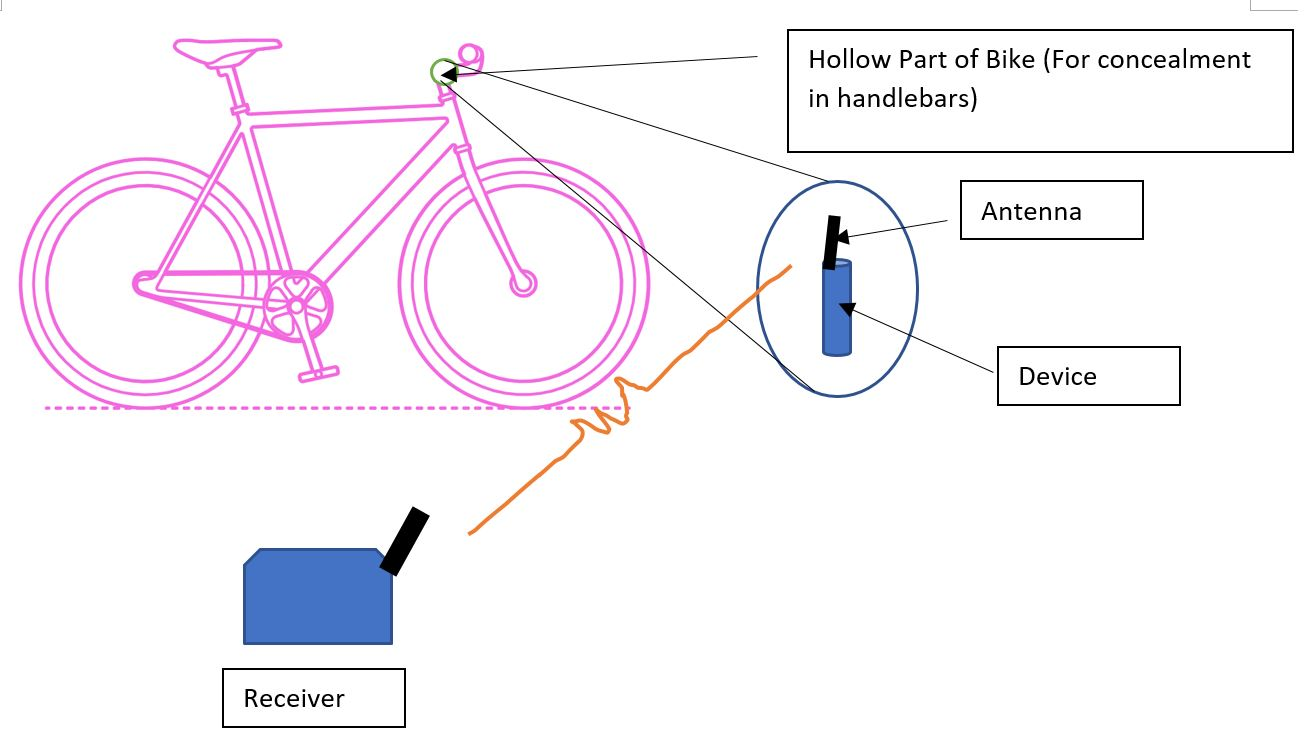
\includegraphics[width=\textwidth]{visual_aid.JPG}
	\caption{Conceptual Diagram}
\end{figure}

\section{Design}
\subsection{Top-Level Block Diagram}

\begin{figure}[H]
	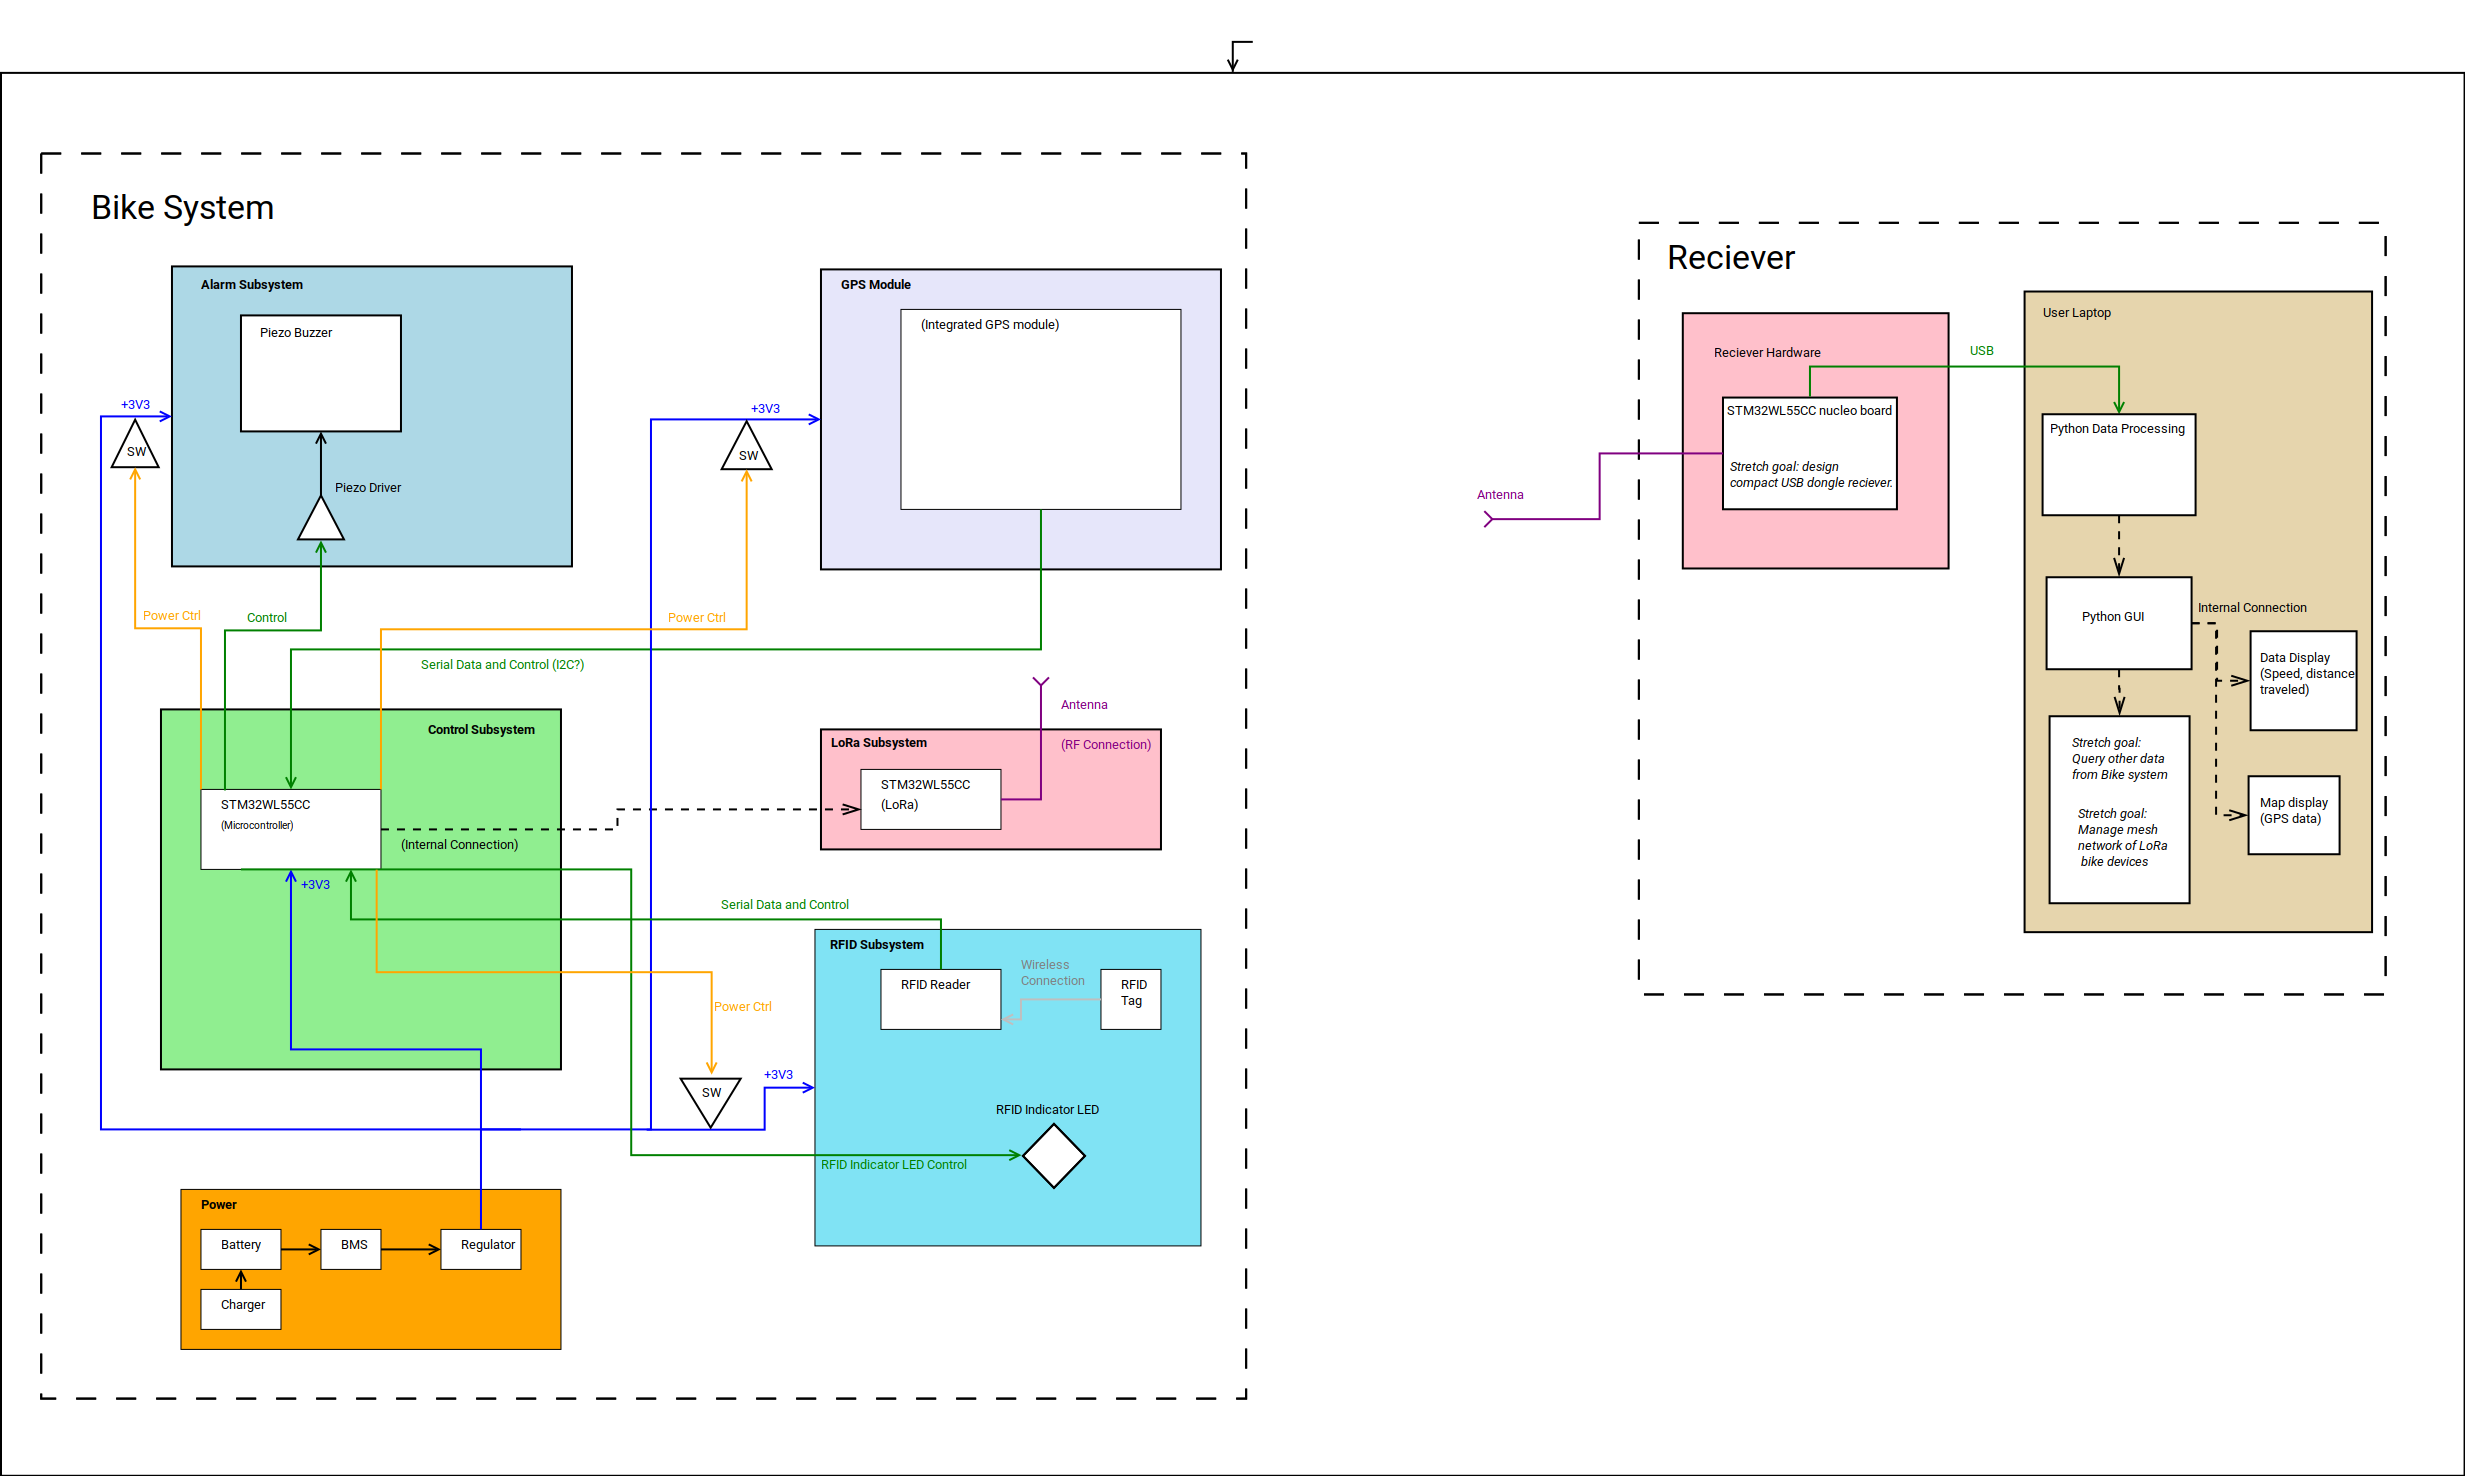
\includegraphics[width=\textwidth]{block_diagram_full.png}
	\caption{Full Block Diagram}
\end{figure}

\subsection{High-Level Requirements}

\begin{enumerate}
	\item If a user tries to remove the bike from a stationary location without the RFID tag, the alarm will sound. 
	
	\item The device receives GPS data \textit{at least} once per minute, and records its own position over time.  
	
	\item The device transmits its GPS location data and additional data over LoRa to be received by a base station. 
	
\end{enumerate}

\subsection{Subsystem Overview}
\subsubsection{Control Subsystem}

\paragraph{}
 We will use the STM32WL55CC, an SoC that includes both a dual-core ARM microcontroller and a wireless transceiver \cite{stm_datasheet}. The microcontroller will be responsible for buffering data from the GPS receiver, packetizing the data to send over LoRa, and internally transferring the data to the integrated RF transceiver. The microcontroller will also manage the control signals for the alarm subsystem, RFID subsystem, and GPS module. 

 Since this is a battery-powered device, the microcontroller will also be responsible for implementing power-saving measures. For example, the microcontroller will vary the number of GPS data transmissions depending on the bike state: while the bike is in a “idle/safe” state (stationary in one location) it will only transmit its location over LoRa once per hour. If the device is in the “stolen” state, it will transmit its location over LoRa once per minute. The microcontroller will also cut off power to the Alarm when it is not in use, and as a stretch goal, the microcontroller will selectively cut power to the RFID/GPS subsystems in an intelligent manner (ie, the RFID transmitter will not continuously transmit/listen for the RFID tag if the GPS module detects that the bike is in motion, and the motion was initiated by the correct user). 
\paragraph{} 

\textit{\textbf{Control Subsystem Requirements:}}

\begin{enumerate}
	\item The microcontroller implements a state-based control system with power-saving measures in the idle/safe states. 
	\item The microcontroller packetizes data to be sent over LoRa at an update rate of \textit{at least }once per hour in “idle” states, and \textit{at least} once every two minutes in “active” states. 
	\item \textit{Stretch goal:} The microcontroller manages multi-unit mesh networking by re-transmitting received data within 1 second of receiving the data. (See the \textbf{LoRa Subsystem} section for more detail on mesh networking). 
\end{enumerate}


\subsubsection{LoRa Subsystem}

\paragraph{} We will use LoRa, a low-power spread-spectrum RF protocol, to transmit GPS data from the bike device to be received by the user. LoRa is an ideal choice for this application because it is extremely low-power, has a range of several miles even in crowded city conditions, and does not require any radio licensing to operate \cite{LoRA}. These qualities will enable our device to function for extended periods of time on battery power, allow the signal to be received by the base station for multiple miles, and allow any user to purchase this device and use it without worrying about licensing. 


The LoRa transceiver is integrated with the STM32WL55CC SoC, so the LoRa subsystem will require us to design an external matching network and antenna \cite{matchingAN}. We will choose a compact antenna and conceal it to prevent theft (for example, inside a hollow conventional plastic reflector that can be mounted on the handlebars or seat; refer to figure \ref{reflector} for an example of one type of bike reflector). We will design the matching network to ensure reflected power is within the STM32WL55CC's maximum reflected power parameter.

As a stretch goal, we will implement a rudimentary form of mesh networking between bike tracking devices. Each bike tracker will listen and re-transmit GPS coordinates it receives from other bike trackers -- as a result, the range of the LoRa bike tracker will be dramatically increased, since its GPS coordinates can be received as long as \textit{any} bike tracker is in range instead of only if the base station is in range. 
\paragraph{} 


\textit{\textbf{LoRa Subsystem Requirements:}}

\begin{enumerate}
	\item The LoRa subsystem matching network and antenna have a VSWR of less than 10 at the RF output of the STM32WL55CC. 
	\item The antenna is hidden in a common bike component such as a reflector so that it is not visibly obvious. 
\end{enumerate}



\subsubsection{GPS Module}

We will use an off-the-shelf GPS module to receive GPS data. We will choose a GPS module that can receive GPS updates at a rate of at least 1 Hz. We will mount the GPS module on the bike such that the GPS antenna is able to see a clear view of the sky, but is concealed from the casual observer. We will likely conceal the small patch antenna inside of a plastic bike reflector such as the type shown below. \footnote{We are not sure if bike reflectors have metal foil inside the plastic -- if this is the case we will obviously remove the metal foil before mounting the antenna.}

\begin{center}
\begin{figure}[H]
	\centering
	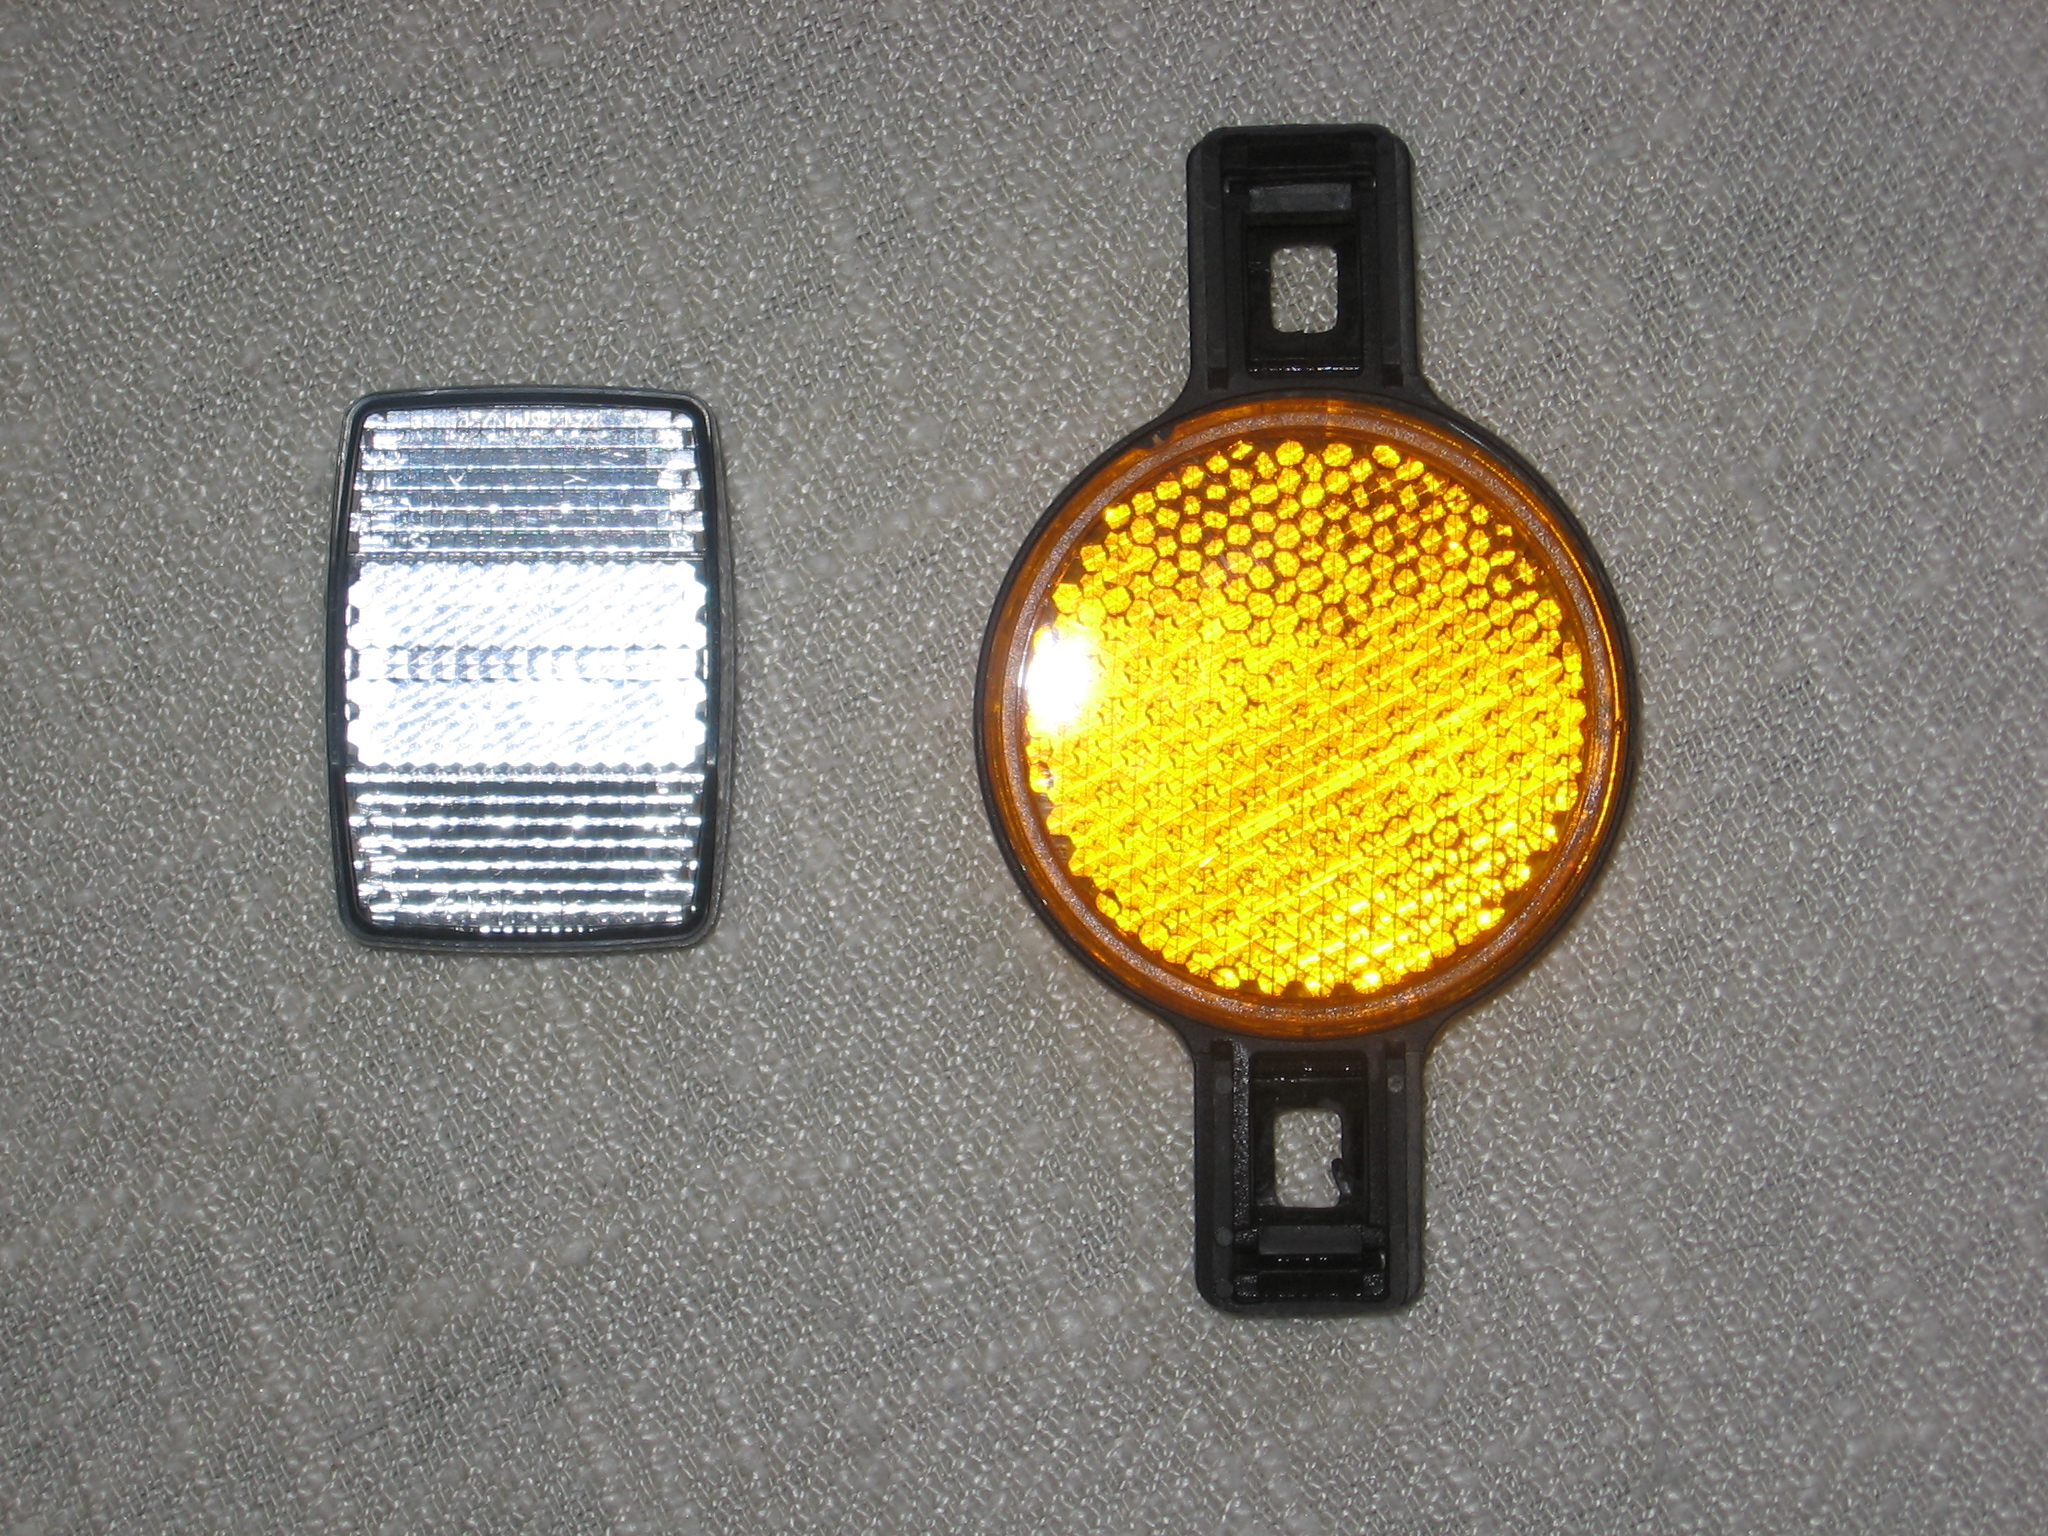
\includegraphics[width=0.25 \textwidth]{bike_reflector.jpg}
	\caption{Example of a plastic bike reflector.} \label{reflector}
\end{figure}
\end{center}


\paragraph{} 


\textit{\textbf{GPS Subsystem Requirements:}}

\begin{enumerate}
	\item The GPS module can communicate with the microcontroller at a update rate of greater than 1 Hz. 
\end{enumerate}	


\subsubsection{RFID Subsystem}


\paragraph{} We will use an off-the-shelf RFID tag and an RFID reader module. The RFID module will listen to determine if the bike owner's RFID tag is present, and transfer the RFID data to the microcontroller. The microcontroller must be able to read the RFID identifier from the transferred data to determine if the owner's RFID tag is present (so that the device does not just trigger when any RFID is present). 

To increase ease of use, we will include a visual indicator such as a concealed LED to show whether or not the correct RFID tag has been detected so that the user doesn't accidentally set off the alarm. The visual indicator will be concealed in a common bike component or unobtrusive location. 

\paragraph{} 


\textit{\textbf{RFID subsystem requirements:}}
\begin{enumerate}
	\item The RFID detector will detect the user’s RFID tag within 10 seconds. 
	\item The RFID subsystem will provide a visual indication that the RFID tag has been detected within 1 second of detecting the RFID tag. 
	\item The RFID subsystem does not disable the alarm unless the user's RFID is detected.
	\item The RFID indicator LED is concealed in an unobtrusive location on the bike.
\end{enumerate}

\subsubsection{Power Subsystem} 

We will power the device with three AA batteries in series to provide approximately 2700 mAh at 4.5V \cite{battery}. We will implement a basic battery management system to ensure the batteries do not reach an unsafe state. As a stretch goal, we will include USB-C recharging capabilities. We will use linear regulators to provide a smooth 3V3 supply voltage for all subsystems. 
\paragraph{} 

\textit{\textbf{Power subsystem requirements:}}

\begin{enumerate}
	\item The power system will provide 3V3 $\pm$ 0.4 mV to all subsystems. 
	\item The power system will power the device for over 24 hours. 
\end{enumerate}

\subsubsection{Alarm Subsystem} 

We will use a simple Piezo buzzer as the alarm. The alarm will be driven by the driver circuit shown in figure \ref{buzzer}. As shown in the diagram, when the FET is turned off, the circuit draws negligible current, thus minimizing power draw. 



\begin{center}
	\begin{figure}[H]
		\centering
		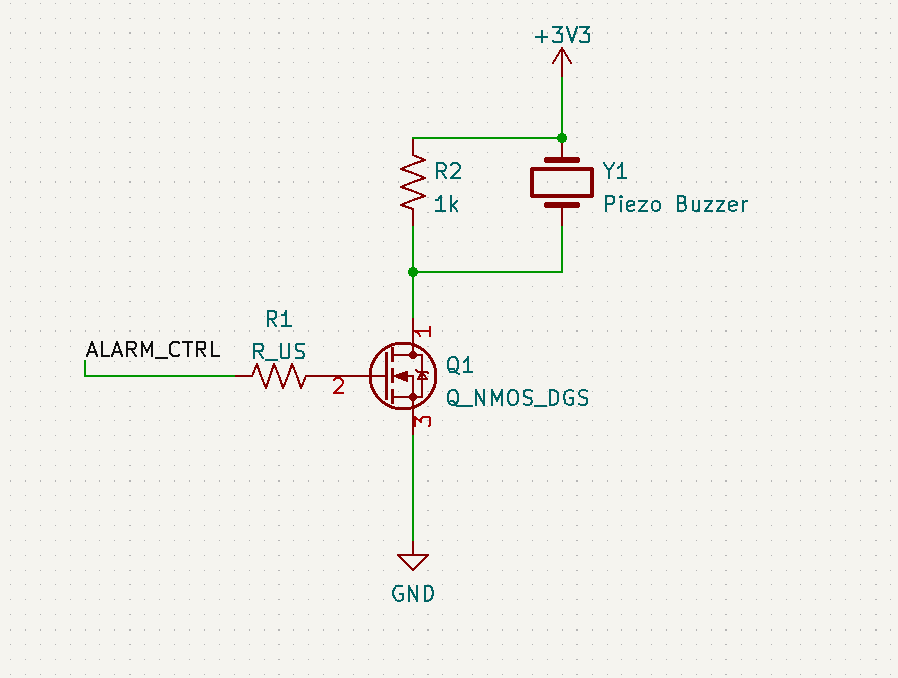
\includegraphics[width=0.25 \textwidth]{buzzer_ckt.png}
		\caption{Basic Piezo buzzer driver circuit.} \label{buzzer}
	\end{figure}
\end{center}


\paragraph{} 

\textit{\textbf{Alarm Subsystem Requirements:}}

\begin{enumerate}
	\item The alarm makes noise when triggered by the ALARM\_CTRL signal. 
	\item The alarm circuit draws < 1 uA of current when not making noise.
\end{enumerate}




\subsubsection{Base Station Subsystem} 

\paragraph{} 
In order for the user to receive the data from the bike system, they will need to have a LoRa receiver. In practice, this could be a commercial off-the-shelf LoRaWAN receiver, but for our purposes, we will use a similar STM32 board as the bike system but running different firmware to interface with a laptop over USB. 

On the laptop, we will implement a GUI to visualize the bike GPS data and view past data. The GUI will plot the GPS location on a map for the user to view. Additionally, the user will be able to view plots of average speed and distance traveled. As a stretch goal, if we are able to implement rudimentary mesh networking, we will plot the location of other bike systems on the map as well and allow the user to access data about any of the bike trackers present in the network. 


\paragraph{} 
\textit{\textbf{Base Station Subsystem Requirements:}}

\begin{enumerate}
	\item The receiver board will receive LoRa packets from the bike-based device. 
	\item The receiver board will interface with the computer over USB.
	\item The GUI will display GPS data over the past day, week, month, or year on a map. 
	\item The GUI will allow the user to view plots of the average speed and distance traveled.
\end{enumerate}


\subsection{Tolerance Analysis}

Since this is a battery-powered device that is meant to be unattended for relatively long periods of time, it is critical that our power system can supply adequate power for the device over a period of time. Our battery pack will provide approximately 2700 mAh, so we must calculate the total current draw for our device to ensure we can source enough power to power the device for an appropriate period of time. \textit{Note:} We have not decided on a specific RFID/GPS module yet, so these are representative estimates from datasheets of possible options. 

\begin{figure}[H]
	\begin{center}
		\begin{tabular}{|c|c|c|c|c|}
			\hline
			\textbf{Subsystem} &  \textbf{Current Drawn} & \textbf{Duty Cycle Estimate} \\
			\hline
			Microcontroller/LoRa, high power TX \cite{stm_datasheet} & 120 mA & 5 \% \\
			\hline
			Microcontroller/LoRa \cite{stm_datasheet}, Idle & 3.45 mA & 100 \% \\
			\hline 
			GPS module \cite{gps} & 50 mA & 100 \% \\
			\hline
			RFID module \cite{rfid} & 45 mA & 100 \% \\ 
			\hline 
			Alarm ON & 3.3 mA & 1 \% \\ 
			\hline
			
		
		\end{tabular}
	\end{center}
	\caption{Power Budget Analysis}
\end{figure}

From the chart above, we can see that the full current drawn during operation (assuming 100\% duty cycle for the RFID and GPS module) is: 

$$ 
120(0.05) \text{ mA}+ 3.45 \text{ mA}+ 50\text{ mA} + 45\text{ mA} + 3.3 \text{ mA}= 107.75 \text{ mA}
$$


Since we will be using linear regulators, we can assume that the current drawn by the load is the same as the current drawn from the battery pack, and do the power calculation in terms of available milliamp-hours. 

Since the 3 AA batteries can provide 2700 mAh: 

$$ 
\frac{2700 \text{ mA}*\text{hours}}{107.75 \text{ mA} } = 25 \text{ hours of operation}
$$


This is acceptable, but ideally, the device would be able to autonomously operate for multiple days without being recharged. We can increase the operation time significantly by limiting the on-time of the RFID and GPS modules. With a duty cycle of 25 \% for both, we can increase the operational time, as shown below: 
\begin{figure}[H]
	\begin{center}
		\begin{tabular}{|c|c|c|c|c|}
			\hline
			\textbf{Subsystem} &  \textbf{Current Drawn} & \textbf{Duty Cycle Estimate} \\
			\hline
			Microcontroller/LoRa, high power TX \cite{stm_datasheet} & 120 mA & 5 \% \\
			\hline
			Microcontroller/LoRa \cite{stm_datasheet}, Idle & 3.45 mA & 100 \% \\
			\hline 
			GPS module \cite{gps} & 50 mA & 25 \% \\
			\hline
			RFID module \cite{rfid} & 45 mA & 25 \% \\ 
			\hline 
			Alarm ON & 3.3 mA & 1 \% \\ 
			\hline
			
			
		\end{tabular}
	\end{center}
	\caption{Power Budget Analysis: Decreased Duty Cycle}
\end{figure}
$$ 
120(0.05)\text{ mA} + 3.45\text{ mA} + 50(0.25) \text{ mA}+ 45(0.25) \text{ mA}+ 3.3 \text{ mA}= 36.5 \text{mA}
$$


$$ 
\frac{2700 \text{ mA}*\text{hours}}{36.5 \text{ mA} } = 74 \text{ hours of operation}
$$


74 hours of operation is still somewhat low, but more reasonable than a single day. As we proceed with the design, we will work to increase the operational time with a single charge even further by implementing power-saving measures on the device, adding another 3-cell battery pack in parallel, or using a higher-capacity battery. 

\section{Ethics and Safety}
This project is designed with IEEE’s code of ethics in mind, and the main point as we work on the project is “to hold paramount the safety, health, and welfare of the public, to strive to comply with ethical design and sustainable development practices, to protect the privacy of others, and to disclose promptly factors that might endanger the public or the environment” \cite{ethics}.

A proponent safety concern among electrical design is the battery. With the consideration of including a rechargeable battery, proper use and design may lead to battery failure - potentially leading up to explosion. As such, we work to limit the risk by ensuring that the amount of power drawn and the cell voltage are maintained within the safety limit of the battery used through the use of a power regulator. We are also making sure that the design accounts for the battery being maintained and operated in safe operating conditions.
Battery Charge/Discharge?

Furthermore, the design is implemented with LoRa and RF identification, which involves the transmitting and receiving of information wirelessly. As such, an ethical consideration that is paramount to our objective is that data is received accurately. This is important because if given false or failed readings thieves can make off with the bike even with the flawed design attached due to failure or misreading of information. As such, we plan to ensure that the correct RFID tag can communicate with the appropriate transmitter such that the alarm will sound if and only if the bike is in motion and reaches out of range of the appropriate RFID. 

\begin{thebibliography}{}
	\bibitem{ethics} IEEE, "IEEE Code of Ethics," \textit{IEEE}, 2022. Available: https://www.ieee.org/about/corporate/governance/p7-8.html. [Accessed: Feb. 10 2022].
	\bibitem{LoRA} LoRa Alliance, "What is LoRaWAN: A Technical Overview of LoRa and LoRaWAN", 2015.
	
	\bibitem{gps} GlobalSat. "GlobalSat GPS Module Hardware Data Sheet." Product No: EM-506. 2013. https://cdn.sparkfun.com/datasheets/GPS/EM506\_um.pdf
	
	\bibitem{rfid} ID-innovations. "ID-3LA, ID-12LA, ID-20LA Low Voltage Series Reader Modules." 2015. https://cdn.sparkfun.com/assets/c/7/0/e/3/DS-11828-RFID\_Reader\_ID-20LA\_\_125\_kHz\_.pdf
	
	\bibitem{reflector} Photograph by Julo, public domain, Wikimedia Commons Available: https://upload.wikimedia.org/wikipedia/commons/b/b1/BicycleRetroreflectors.JPG. [Accessed: Feb 10 2022]. 
	\bibitem{matchingAN} STMicroelectronics, "RF matching network design guide for STM32WL Series", AN5457, 2020. 
	\bibitem{stm_datasheet} STMicroelectronics, "Multiprotocol LPWAN dual core 32-bit Arm® Cortex®-M4/M0+	LoRa®, (G)FSK, (G)MSK, BPSK, up to 256KB Flash, 64KB SRAM", DS13293, 2021.
	
	
	
	\bibitem{battery} Wikipedia, "List of Battery Sizes", 2022. [Online]. Available: https://en.wikipedia.org/wiki/List\_of\_battery\_sizes. [Accessed: 10 Feb 2022]. 
	
	
	
\end{thebibliography}
\end{document}
